\section{Features and User Guide}

\subsection{Dashboard}

\autoref{fig:dashboard} shows our dashboard page. This page allows the user to navigate and pick the action they want to execute. A Verifier will select “Verify Credential” to submit a verification request of a credential, a Credential Holder can view their credentials by clicking “View Credential” and an Issuing Body will click on Issue credential to create smart contracts.

\subsection{Submit Verification Request}

\autoref{fig:verification_req} shows the verification request page. 
Submits verification requests to ResilientDB given contract address and credential ID. Displays a message when a request is submitted successfully and shows an error message if a field is missing. Navigates to the track status of the verification request page when the Track button is clicked.

\subsection{Track Status of Verification Request}

\autoref{fig:verification_status} shows the current status of a verification requests, including
``Verified'', ``Rejected'', ``Pending'', ``Not Found''.

\begin{figure}
    \begin{center}
        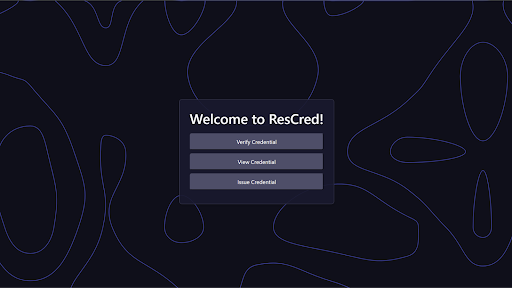
\includegraphics[width=0.95\textwidth]{img/dashboard.png}
    \end{center}
    \caption{ResCred Dashboard}\label{fig:dashboard}
\end{figure}

\begin{figure}
    \begin{center}
        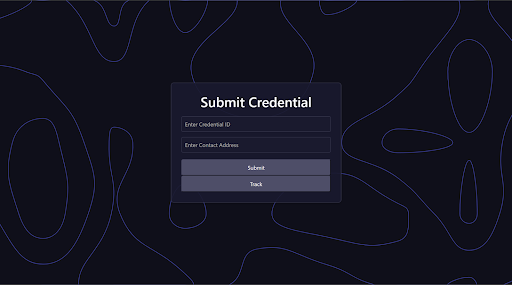
\includegraphics[width=0.95\textwidth]{img/verification_req.png}
    \end{center}
    \caption{Submit Verification Request page}\label{fig:verification_req}
\end{figure}

\begin{figure}
    \begin{center}
        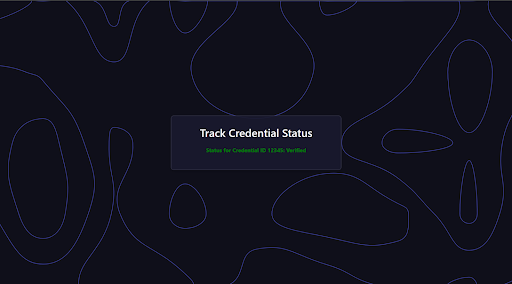
\includegraphics[width=0.95\textwidth]{img/status_verify.png}
    \end{center}
    \caption{Status of Verification Request}\label{fig:verification_status}
\end{figure}


